\begin{frame}
    \frametitle{Why do we need to dissect malware artifacts?}
    \centering

    \bigskip{}

    By looking at the parts, we can understand the whole system
    
    \bigskip{}

    \begin{figure}[!ht]
        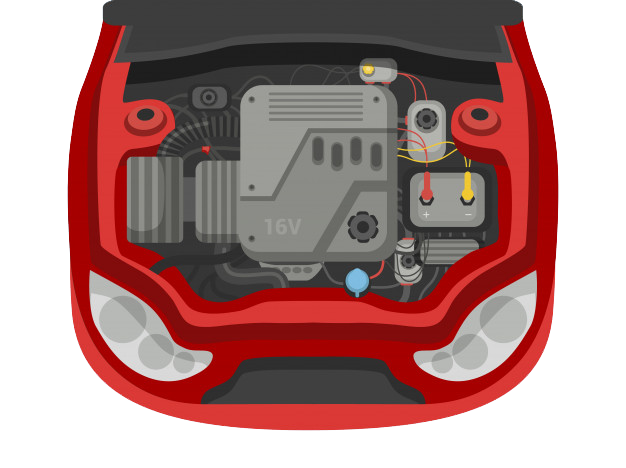
\includegraphics[width=0.75\textwidth]{figures/apgraph/motor.png}
    \end{figure}

\end{frame}

\subsection[AP-GRAPH]{AP-GRAPH:~dissection of malware artifacts}

\begin{frame}
    \vfill
    \centering
    \usebeamerfont{title}

    \begin{beamercolorbox}[sep=8pt,center,shadow=true,rounded=true]{title}
        \textbf{AP-GRAPH}:\\
        dissection of malware artifacts

        \small{}

        \bigskip{}

        \textit{This section is based on unpublished material}
    \end{beamercolorbox}

\end{frame}

\begin{frame}
    \frametitle{Reminders and methodology}

    \begin{columns}
        \begin{column}{0.8\textwidth}
            \begin{block}{}
                \centering
                \textbf{Reminders}
            \end{block}
            \begin{itemize}
                \item Antivirus labels lack proper descriptions
                \begin{itemize}
                    \item e.g., triggers, activities, monetization \ldots
                \end{itemize}
                \item Experts need to know what malware do
                \item How can we materialize malicious behaviors?
            \end{itemize}

            \begin{block}{}
                \centering
                \textbf{Methodology}
            \end{block}
            \begin{itemize}
                \item Focus on artifacts specific to malware family
                \item Implement our approach on a large scale set
                \item Evaluate their practical use in several cases:
                \begin{itemize}
                    \item characterization, localization, and monitoring
                \end{itemize}
            \end{itemize}
        \end{column}

        \begin{column}{0.3\textwidth}
            \begin{figure}[!ht]
                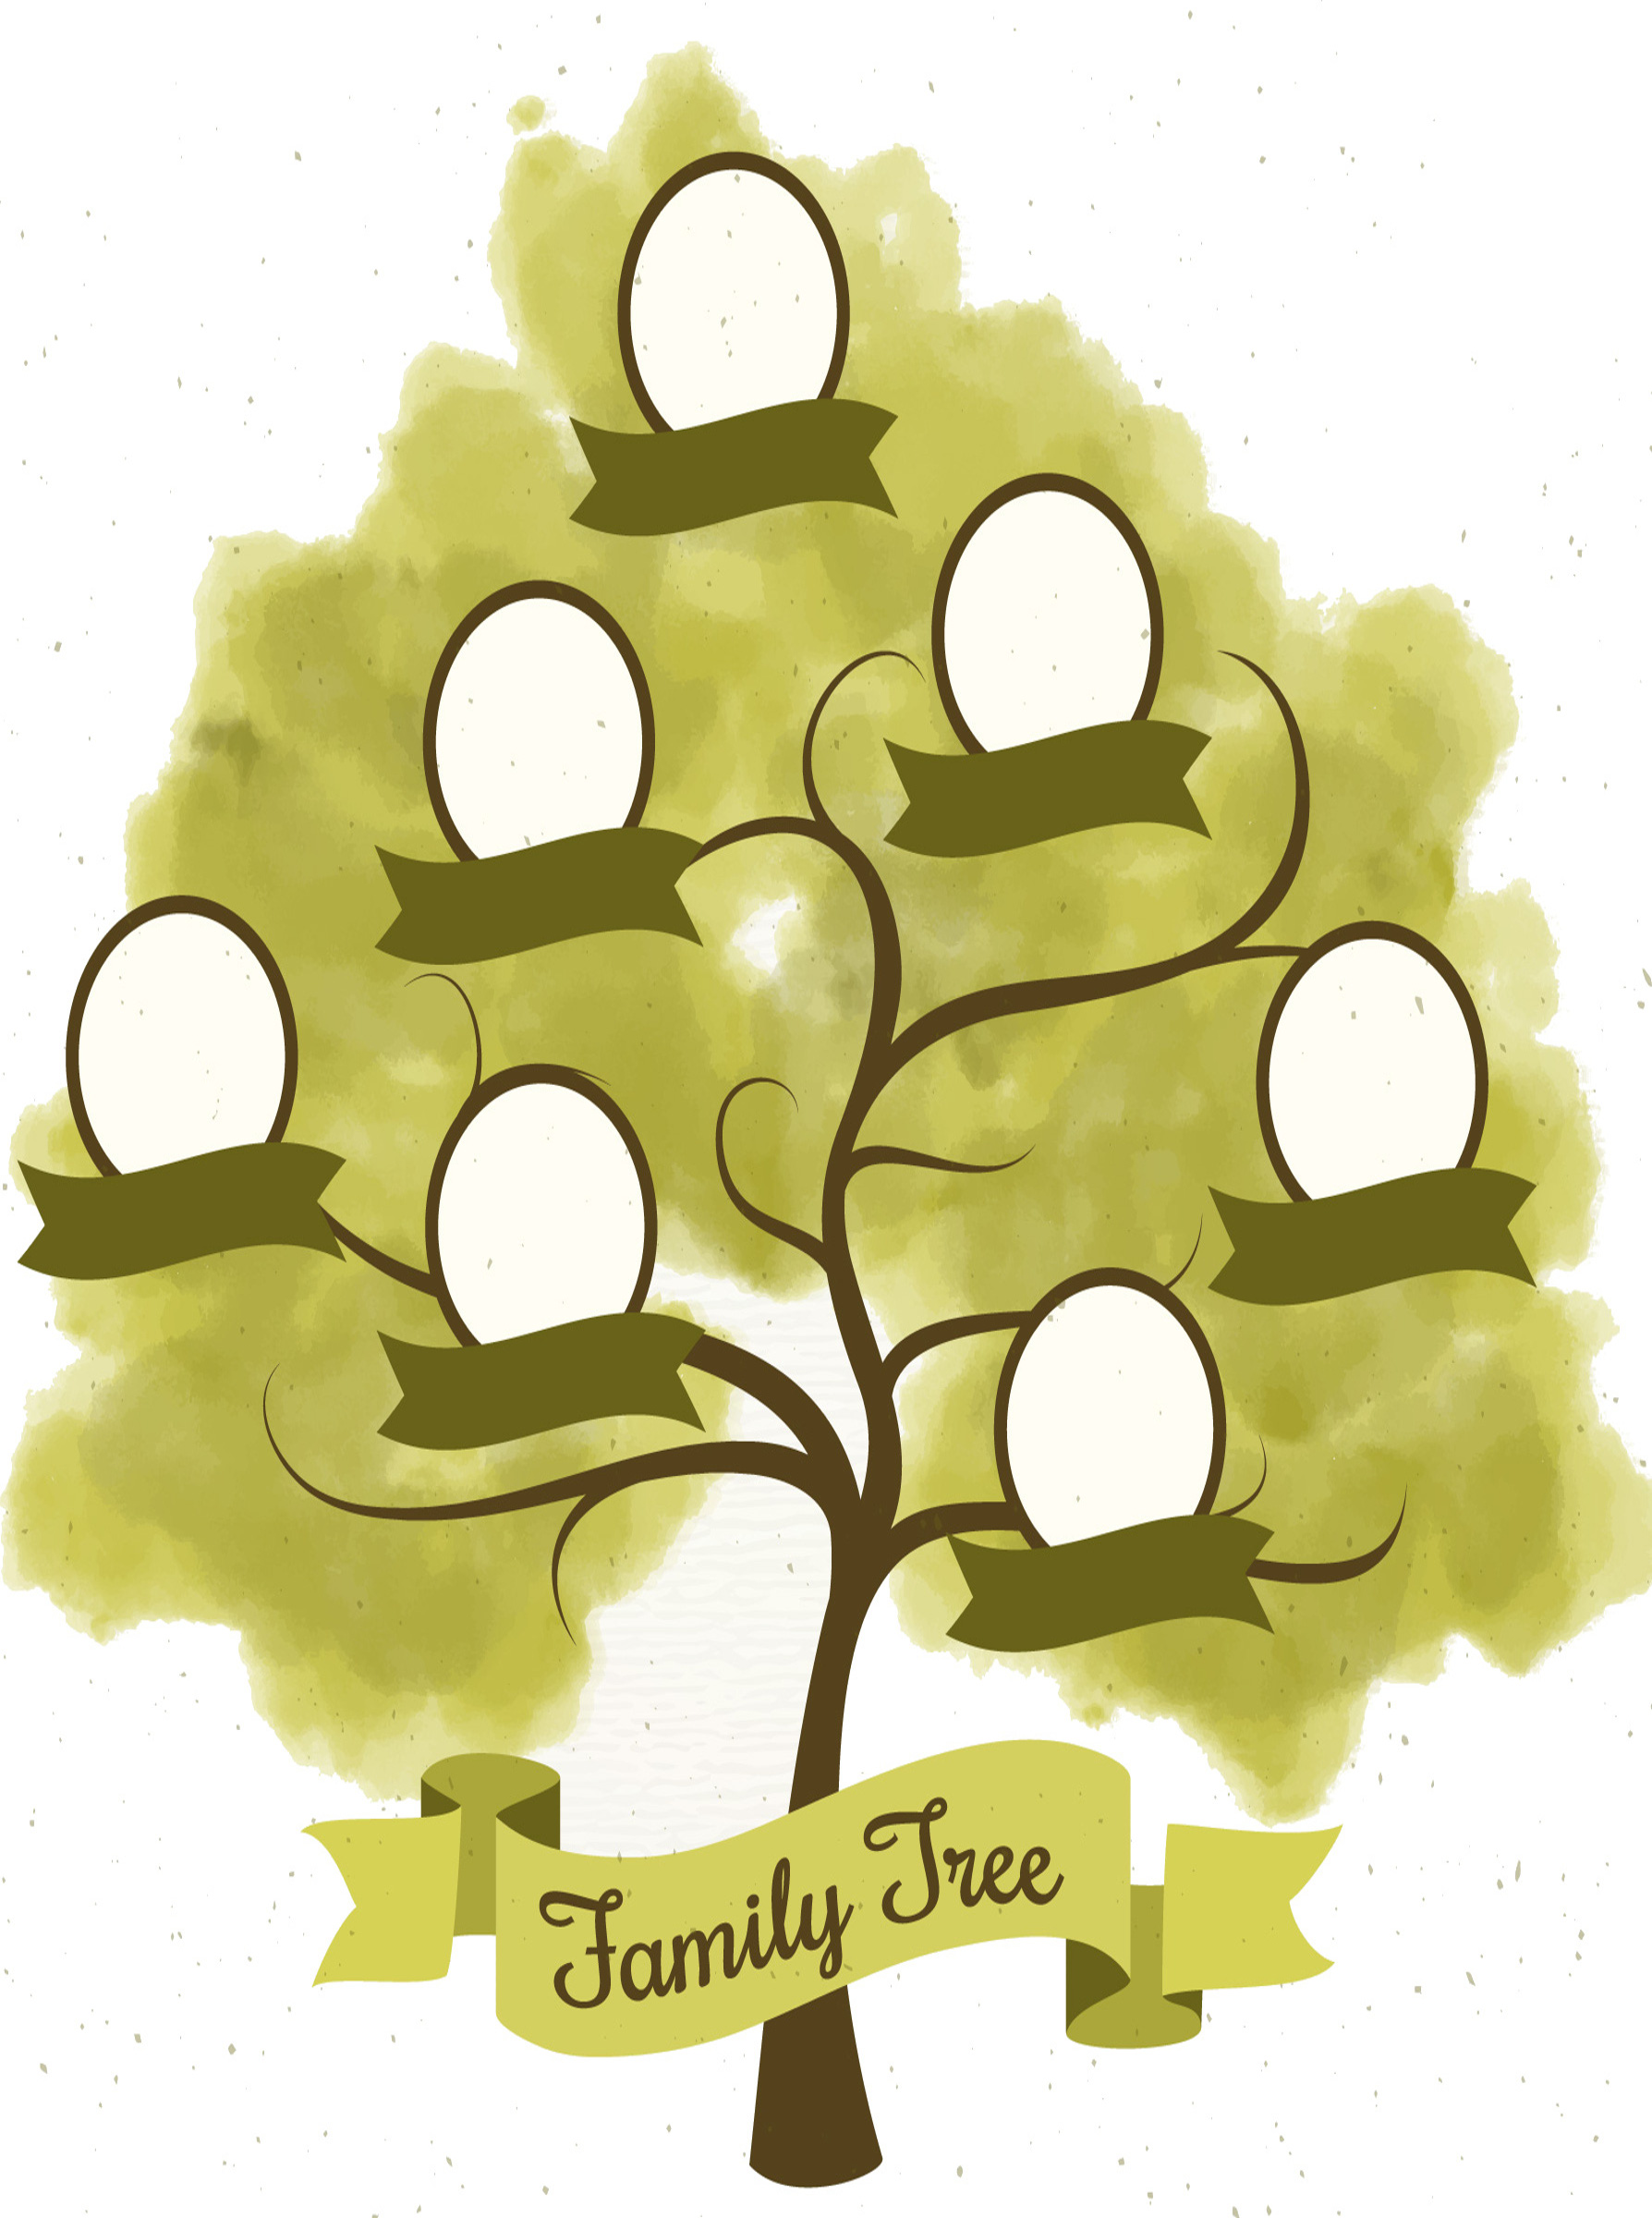
\includegraphics[width=0.95\textwidth]{figures/apgraph/tree.jpg}
            \end{figure}
        \end{column}
    \end{columns}

\end{frame}

\begin{frame}
    \frametitle{Relation graph between applications and artifacts}
    \centering

    \textit{method:loadJava} is not specific either to DOWGIN or KUGUO \\

    \begin{figure}[!ht]
        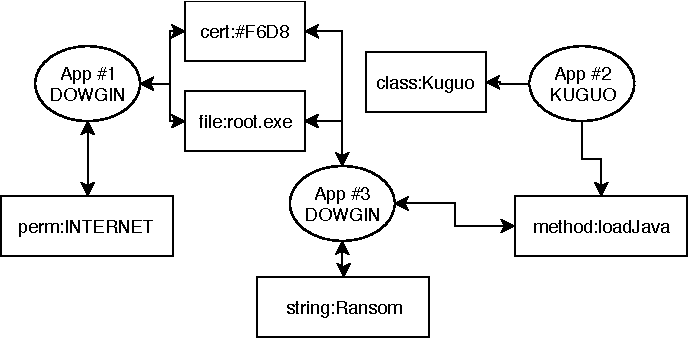
\includegraphics[width=0.95\textwidth]{figures/apgraph/structure.pdf}
    \end{figure}

    But other artifacts can be associated with these families \\
    \smallskip{}
    e.g., \textit{class:Kuguo}, \textit{file:root.exe}, \textit{string:Ransom} \ldots

\end{frame}



\begin{frame}
    \frametitle{Identify artifacts specific to malware families}
    \centering

    $\mathcal{S}(\mathit{g}, \mathit{a}) = \max(\{in(\mathit{g}, \mathit{f}, \mathit{a})~ :~ f~ \in~ fams(\mathit{g}, \mathit{a})\})~ /~ apps(\mathit{g}, \mathit{a})$ \\
    \smallskip{}
    \small{
        where $\mathit{g}$ is a relation graph, $\mathit{a}$ is an artifact and $\mathit{f}$ is a family
    }

    \smallskip{}

    \begin{figure}[!ht]
        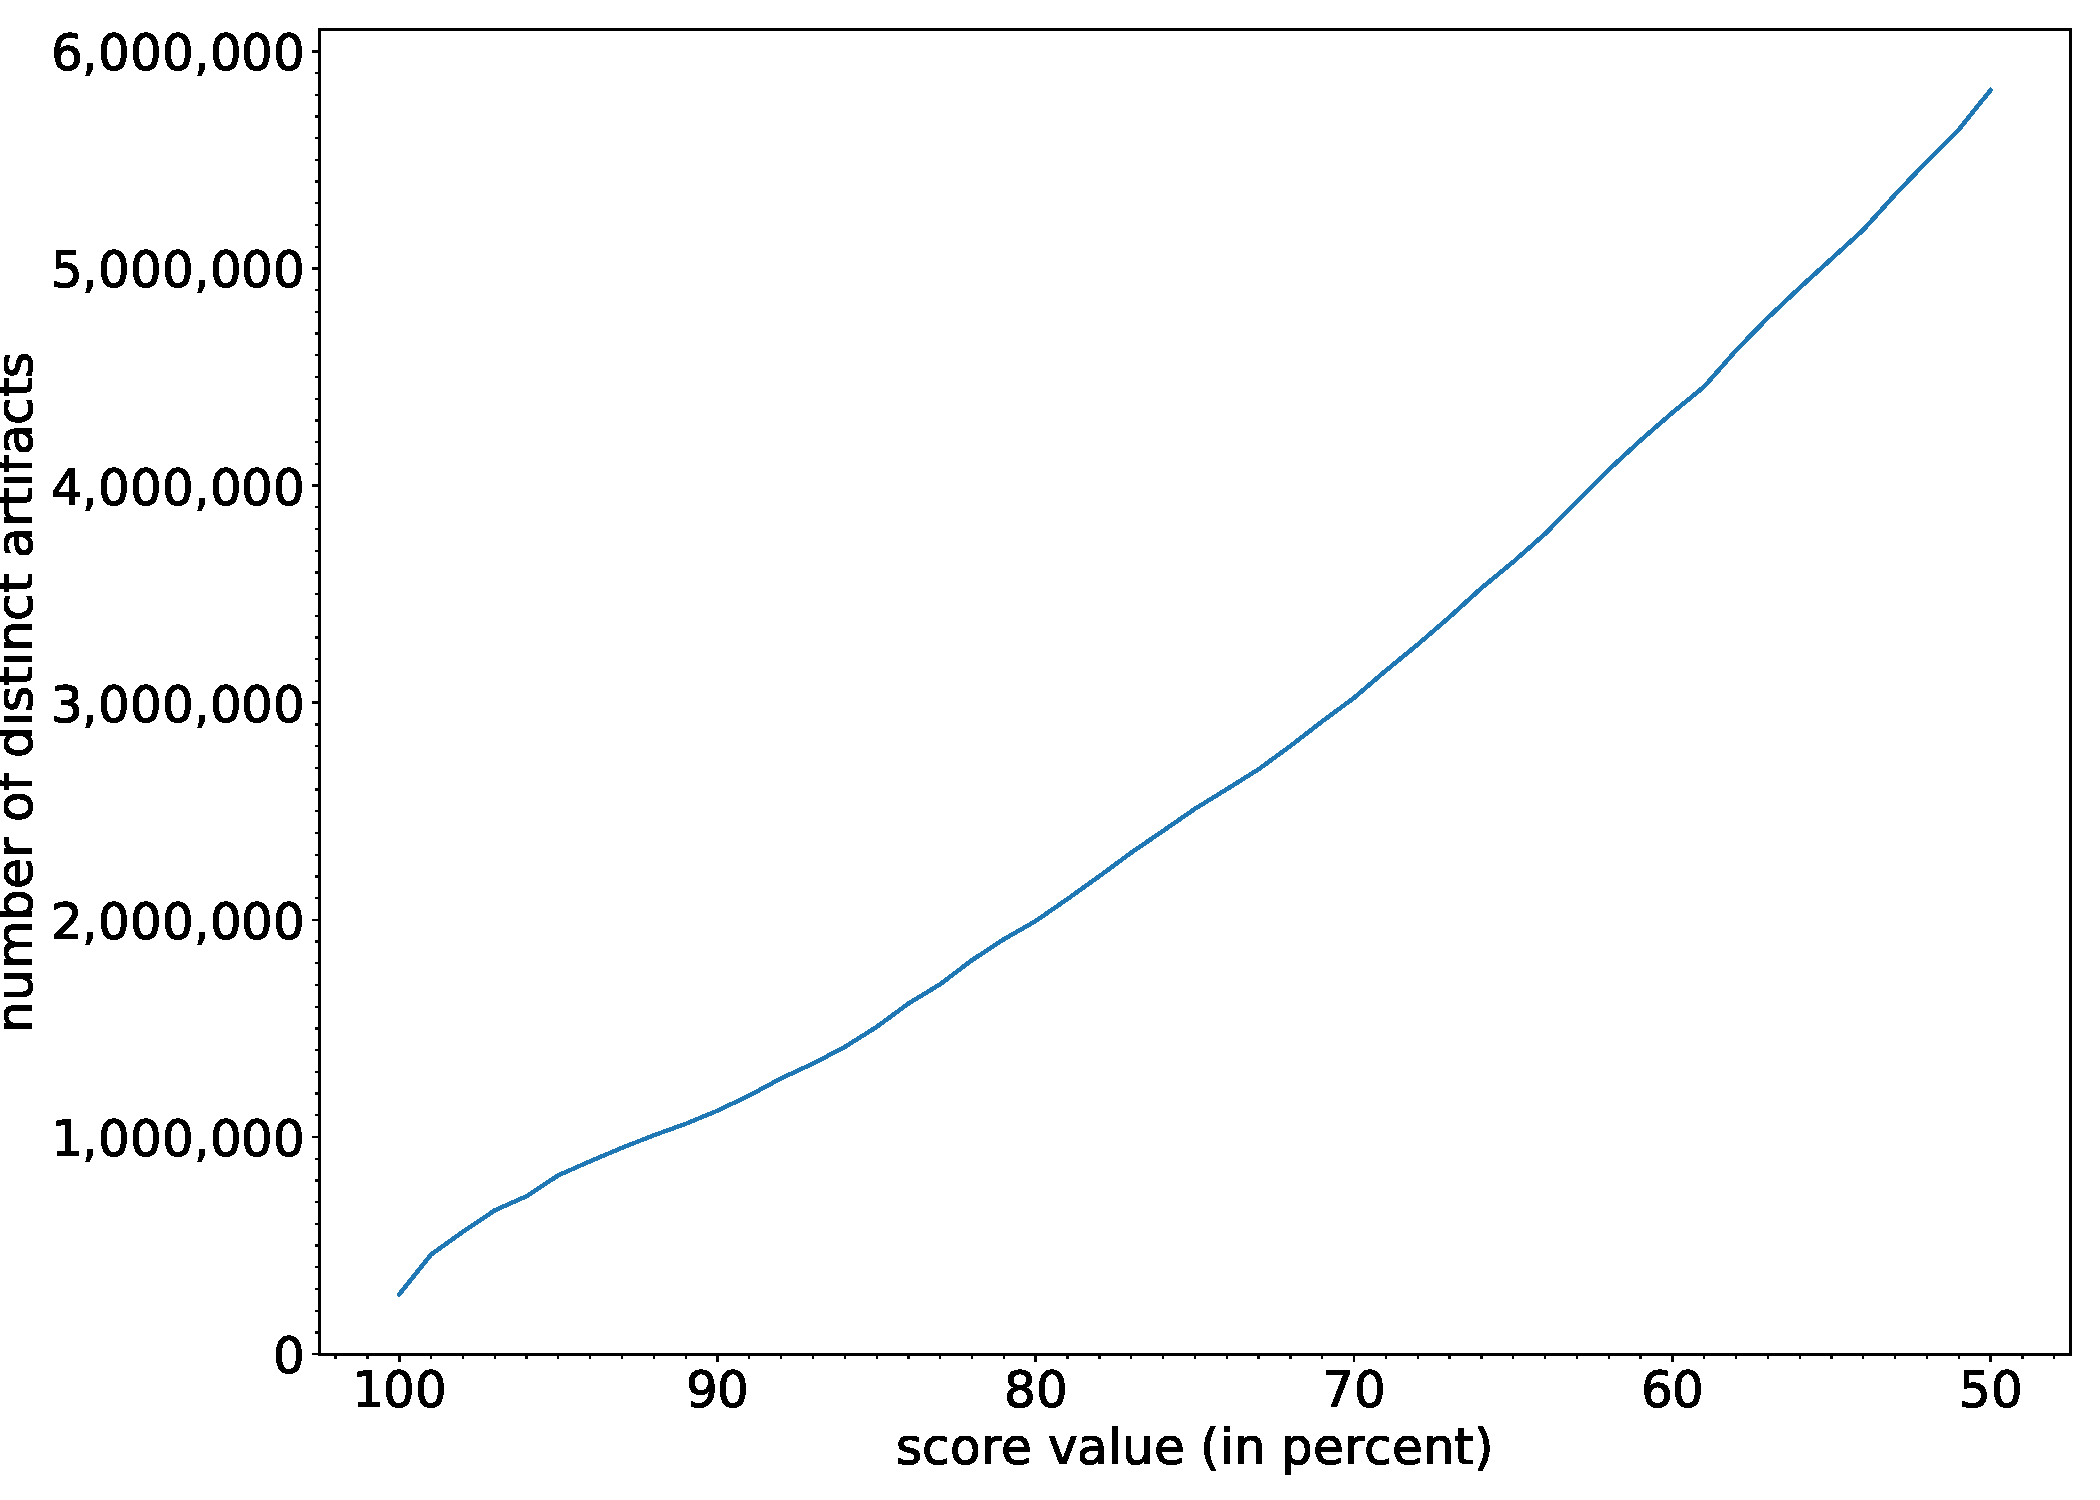
\includegraphics[width=0.58\textwidth]{figures/apgraph/parameters.pdf}
        \caption{
            \footnotesize{
                Number of distinct artifacts retrieved when $\mathcal{S}(\mathit{g}, \mathit{a}) \geq$ score value (in \%)
            }
        }
    \end{figure}

    \vspace{-10pt}

    The goal is to \textit{maximize} the number of artifacts retrieved \\
    while \textit{minimizing} the approximation error $\sum (1 - S(g, a))$

\end{frame}

\begin{frame}
    \frametitle{Implementation of AP-GRAPH based on flat files}

    \begin{figure}[!ht]
        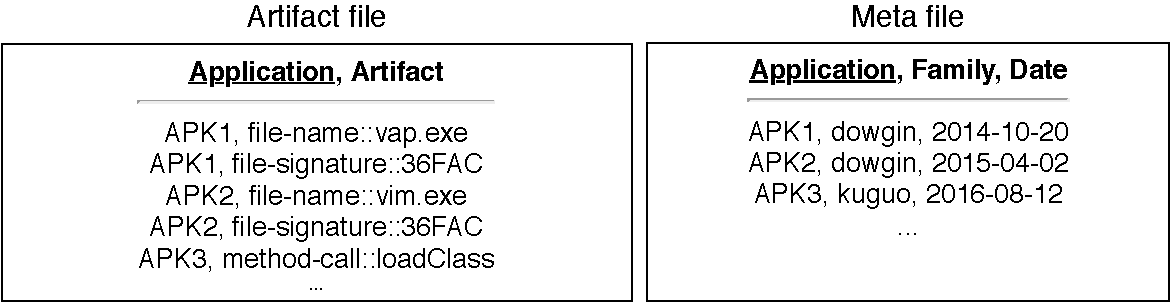
\includegraphics[width=\textwidth]{figures/apgraph/implementation.pdf}
        \caption{\footnotesize{Structure of a relation graph of artifacts implemented with flat files}}
    \end{figure}

    \vspace{-5pt}

    \begin{block}{}
        \centering
        \textbf{Algorithm}
    \end{block}

    \begin{enumerate}
        \item Initially, artifact file is sorted based on the application key
        \item Artifacts are indexed by sorting the file on the artifact key
        \item Statistics are computed by aggregating consecutive values
    \end{enumerate}

\end{frame}

\begin{frame}
    \frametitle{Datasets and characterization of malware families}
    \centering

    \normalsize{Our evaluation is performed on \textbf{1 million} malware of Androzoo} \\
    \smallskip{}
    \small{We report the results of the top 20 families and 5 antivirus}

    \begin{columns}
        \begin{column}{0.5\textwidth}
            \begin{figure}[!ht]
                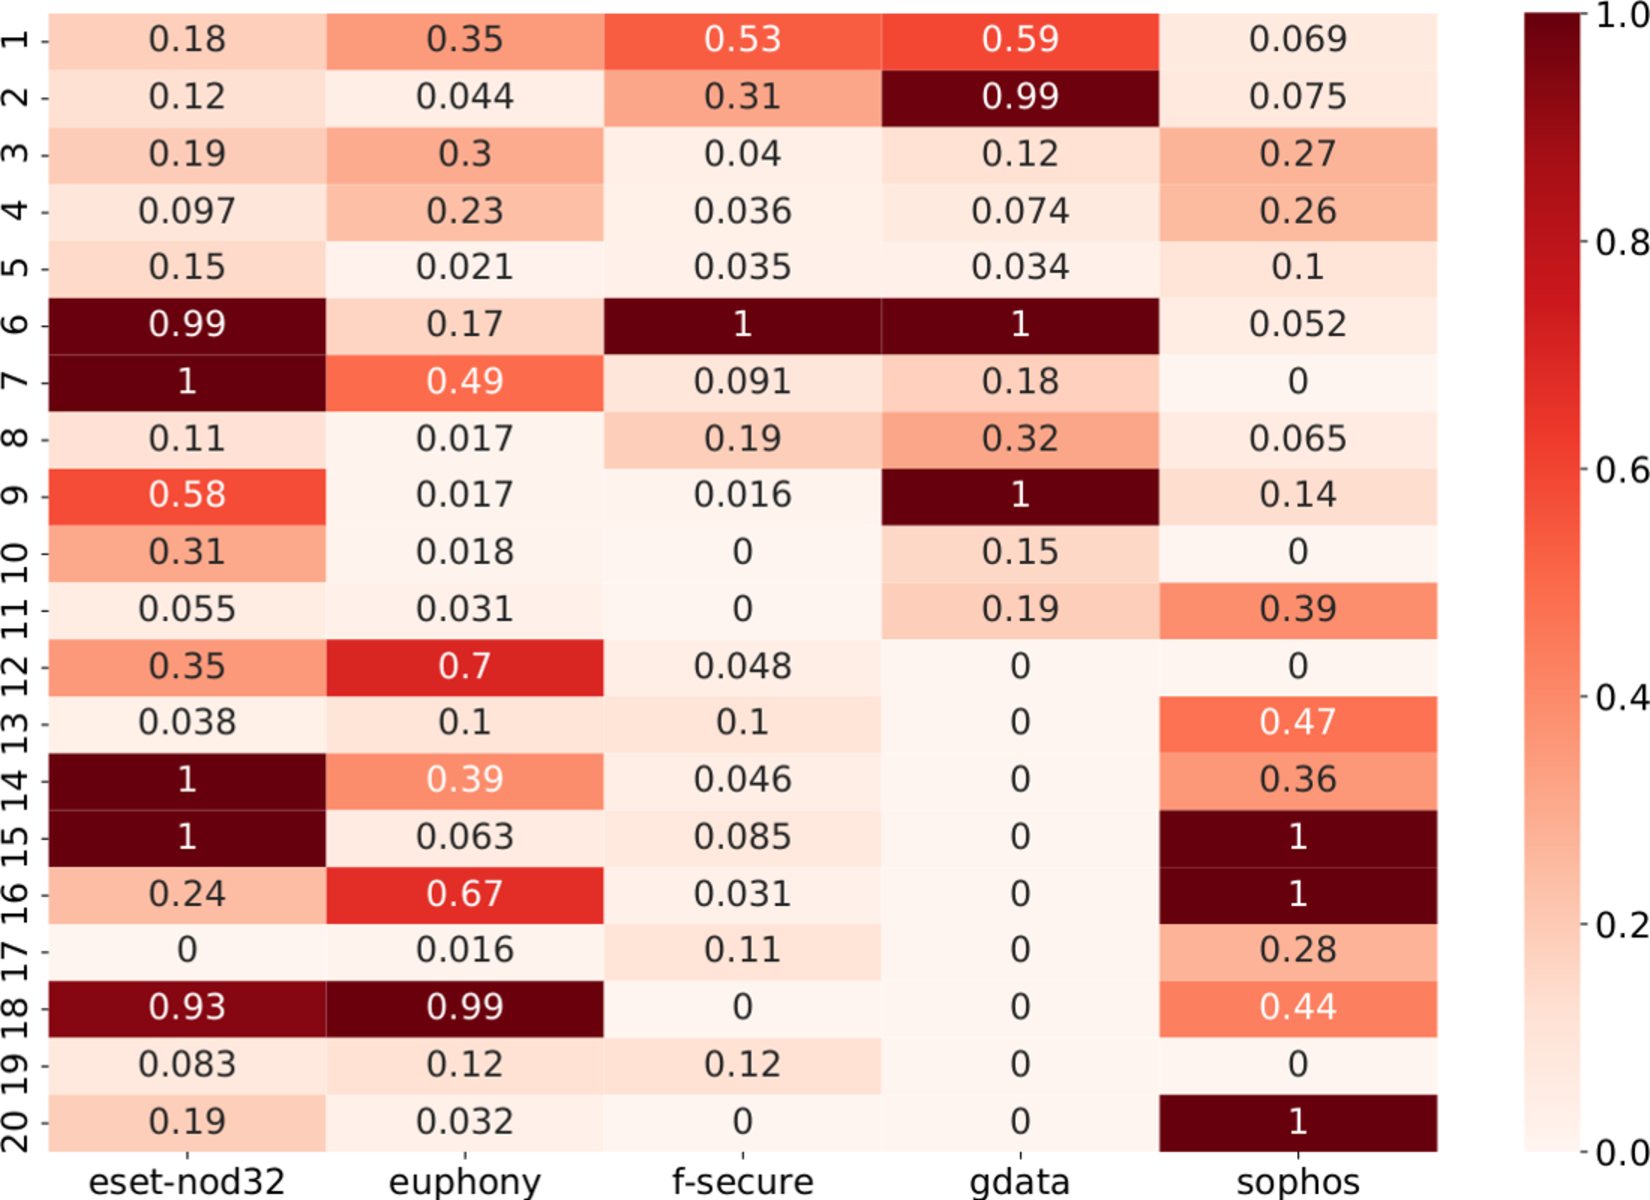
\includegraphics[width=\textwidth]{figures/apgraph/results/proportions.pdf}
                \caption{\scriptsize{Proportion of malware identified}}
            \end{figure}
        \end{column}

        \begin{column}{0.5\textwidth}
            \begin{figure}[!ht]
                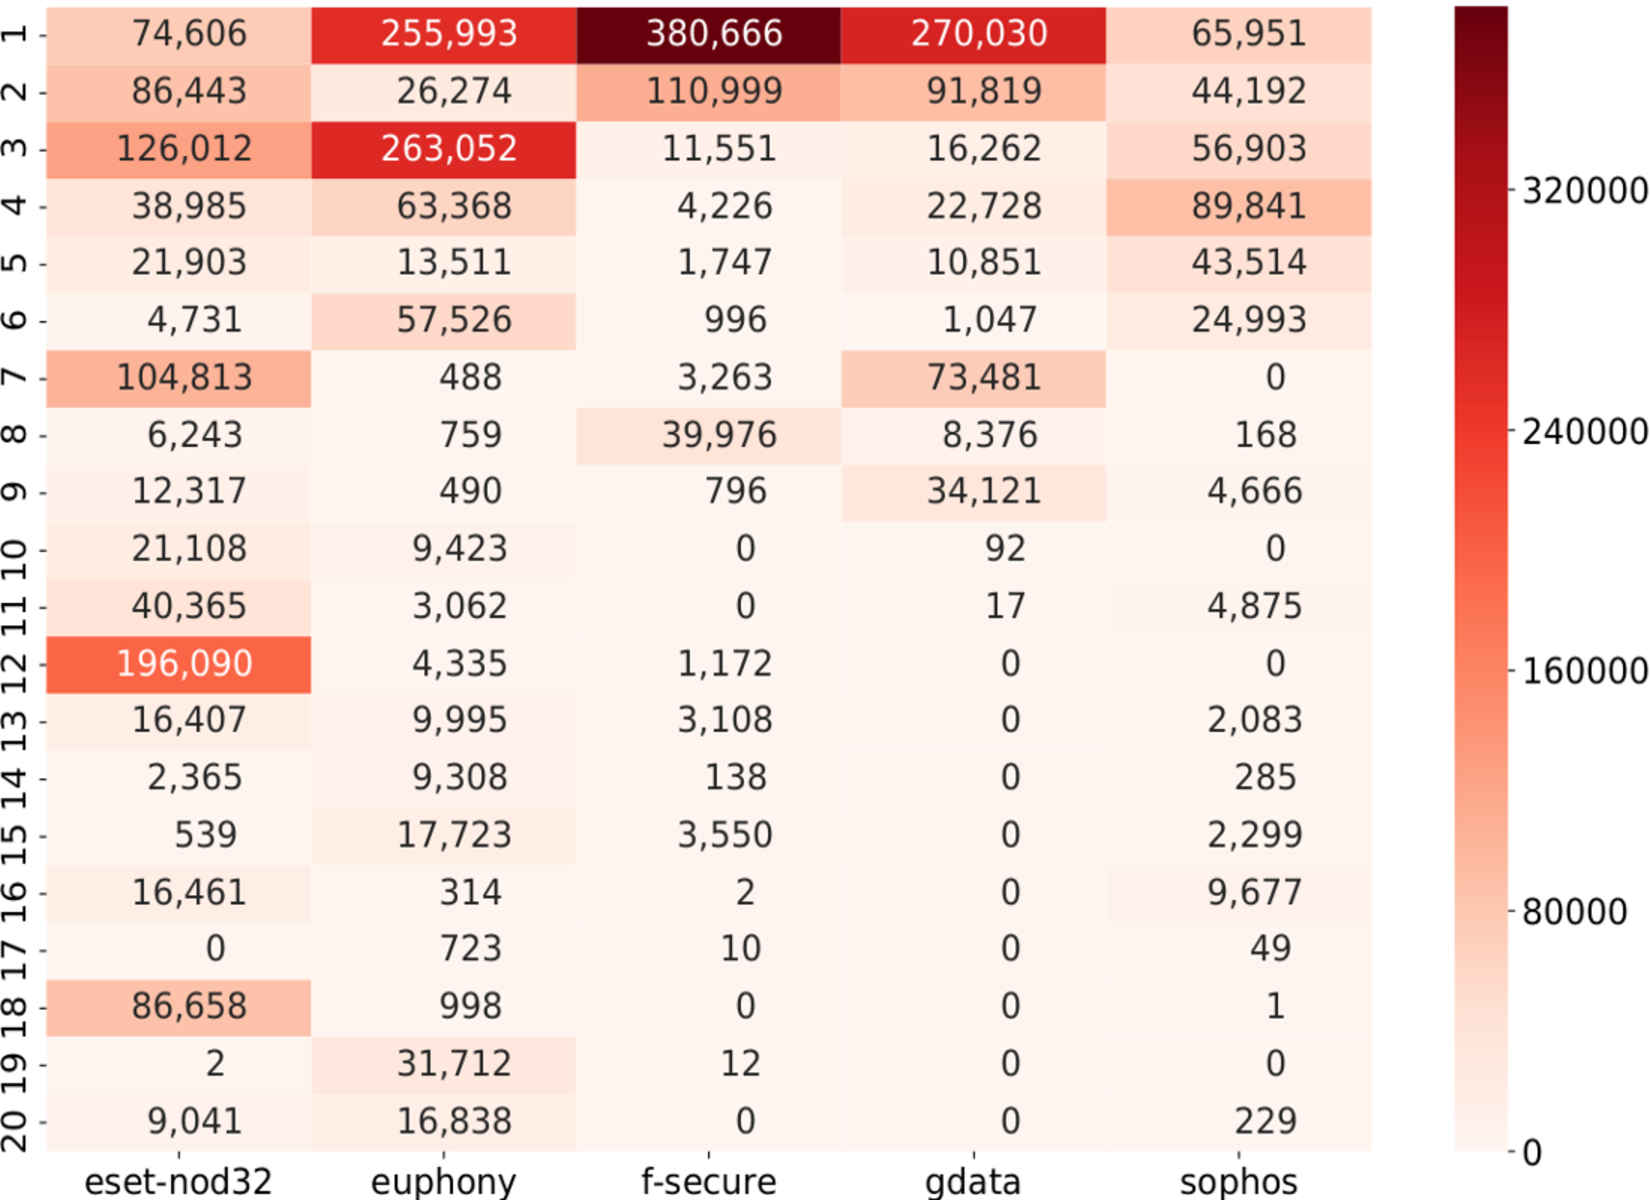
\includegraphics[width=\textwidth]{figures/apgraph/results/numbers.pdf}
                \caption{\scriptsize{Number of artifacts identified}}
            \end{figure}
        \end{column}
    \end{columns}

    \smallskip{}

    \normalsize{Our study includes \textbf{732 million} distinct artifacts in total} \\
    \smallskip{}
    \small{e.g., strings, permissions, method invocations, file signatures \ldots}

    % \item 732 million artifacts in total
    % \item 12 families perfectly identified
    % \item 39 cases with $\geq$ 10,000 artifacts
    % \item 18 cases with 0 artifact retrieved

\end{frame}

\begin{frame}
    \frametitle{Localization of suspicious artifact in the \textit{adwo} family}
    \centering
    \vspace{-20pt}

    \begin{table}[t]
        \resizebox{\textwidth}{!}{
            \begin{tabular}{|c|c|c|r|}
    \hline
    \textbf{Location} & \textbf{Type} & \textbf{Value} & \textbf{found} \\
    \hline
    manifest & activity & \textbf{adwoadbrowseractivity}                            & 44,162 \\
    dex      & invoke   & com/adwo/adsdk/i-><init>                                  & 33,889 \\
    dex      & invoke   & com/adwo/adsdk/h-><init>                                  & 33,078 \\
    dex      & class    & FSAd                                                      & 32,551 \\
    dex      & invoke   & com/adwo/adsdk/AdwoSplashAdActivity->requestWindowFeature & 32,541 \\
    dex      & invoke   & \textbf{com/adwo/adsdk/AdwoSplashAdActivity->getWindow}   & 32,541 \\
    dex      & string   & lcom/adwo/adsdk/fsad;                                     & 32,536 \\
    dex      & code     & \#583b5                                                   & 32,536 \\
    dex      & invoke   & com/adwo/adsdk/FSAd-><init>                               & 32,536 \\
    dex      & string   & \textbf{http://r2.adwo.com/adfs}                          & 32,518 \\
    dex      & string   & vlijlzzz                                                  & 32,505 \\
    dex      & code     & \#1b25f                                                   & 32,485 \\
    dex      & invoke   & com/adwo/adsdk/V-><init>                                  & 32,268 \\
    dex      & code     & \#baf7b                                                   & 32,103 \\
    dex      & string   & malformed click url.will try to follow anyway.            & 32,093 \\
    dex      & invoke   & com/adwo/adsdk/AdwoAdBrowserActivity->a                   & 32,090 \\
    dex      & string   & \textbf{fsad.htmlcontent}                                 & 32,090 \\
    \hline
\end{tabular}

        }
        \caption{\footnotesize{Specific artifacts identified for the family \textit{adwo} and the antivirus \textit{gdata}}}
    \end{table}

    \vspace{-10pt}

    Experts can leverage the information AP-GRAPH provides \\
    to focus their attention on the most interesting artifacts

\end{frame}

\begin{frame}
    \frametitle{Evolution of malware artifacts for the \textit{Igexin} family}
    \centering

    \begin{figure}[!ht]
        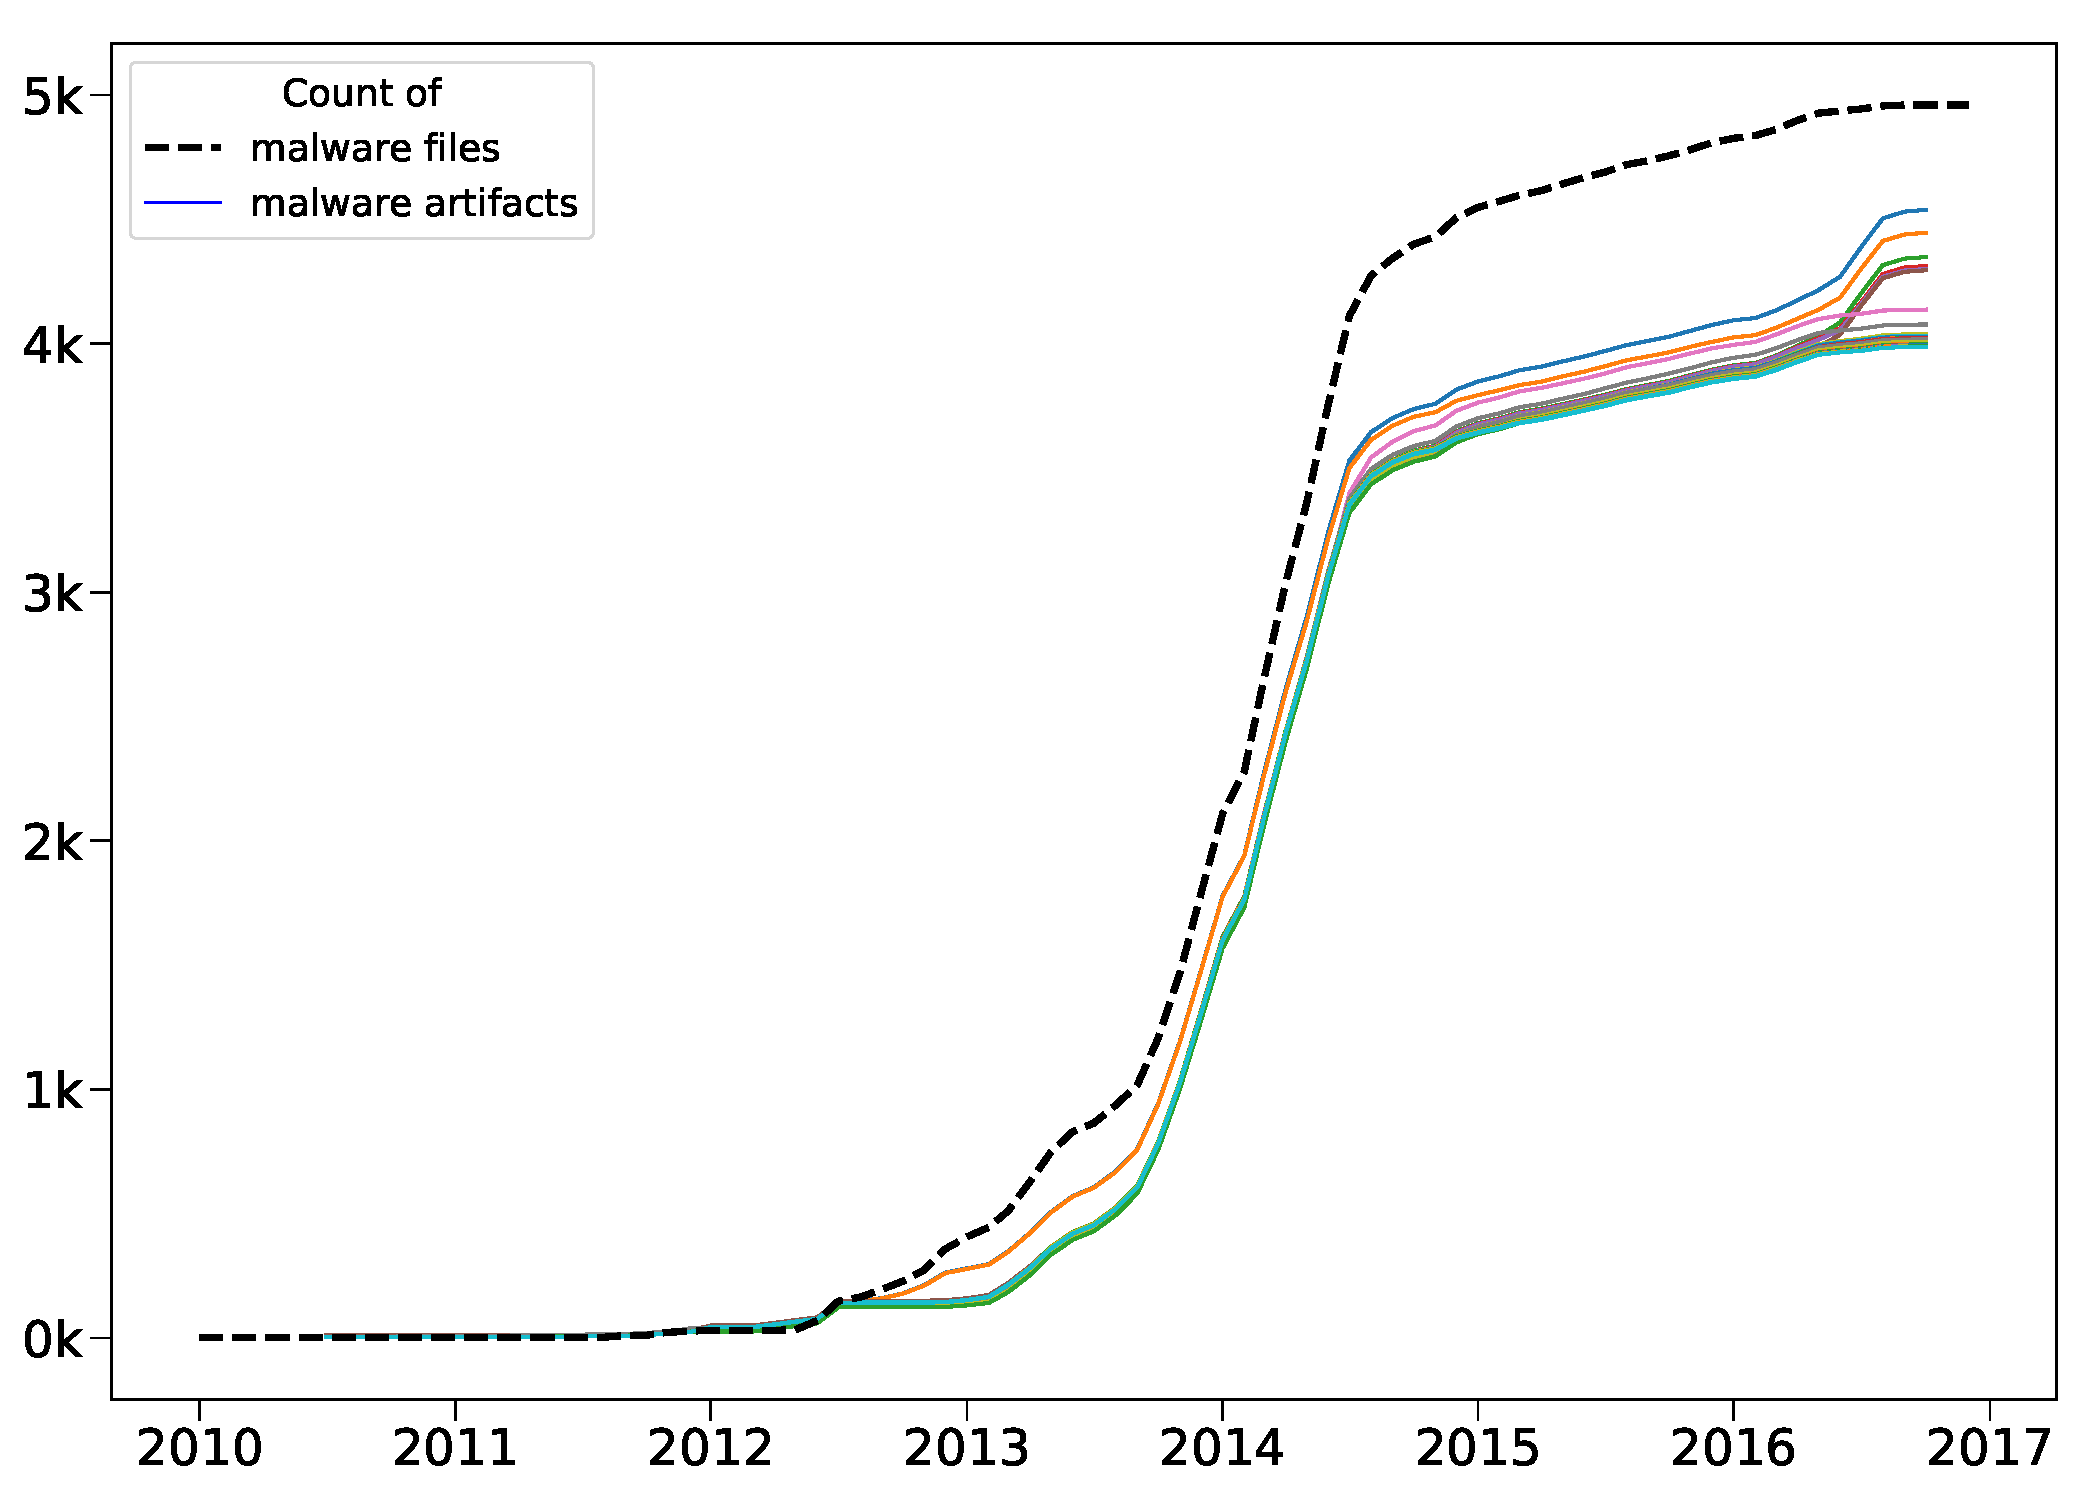
\includegraphics[width=0.75\textwidth]{figures/apgraph/igexin.pdf}
        \caption{\scriptsize{Evolution of the \textit{Igexin} family (dotted line) and 60 of its artifacts (other lines)}}
    \end{figure}

    \vspace{-15pt}

    AP-GRAPH revealed an interesting pattern about the family \\
    \small{i.e., similarity between 2012 and 2014, strong gap afterward}

\end{frame}

\begin{frame}
    \frametitle{Contributions and limitations}

    \begin{block}{}
        \centering
        \textbf{Contributions}
    \end{block}
    \begin{itemize}
        \item Describe malware from the family artifacts
        \item Visualize the evolution of malicious artifacts 
        \item Localize artifacts specific to malware families 
    \end{itemize}

    \begin{block}{}
        \centering
        \textbf{Limitations}
    \end{block}
    \begin{itemize}
        \item Obfuscations and transformations can impair our approach
        \item Benign apps could be included to prevent false positives
        \item AP-GRAPH reveals the correlation, not the causation
    \end{itemize}

\end{frame}
